%%%%%%%%%%%%%%%%%%%%%%%%%%%%%%%%%%%%%%%%%%%%%%%%%%%%%%%%%%%%%%%%%%%%%%%%
% Plantilla TFG/TFM
% Universidad de Murcia. Facultad de Informática
% Realizado por: José Manuel Requena Plens
% Modificado: Pablo José Rocamora Zamora
% Contacto: pablojoserocamora@gmail.com
%%%%%%%%%%%%%%%%%%%%%%%%%%%%%%%%%%%%%%%%%%%%%%%%%%%%%%%%%%%%%%%%%%%%%%%%


\chapter{Análisis de objetivos y metodología}

\section{Objetivos}
El objetivo general de este proyecto es optimizar y acelerar el proceso de generación de tomogramas sintéticos para el \textit{framework} \textbf{PolNet}. Específicamente, se busca perfeccionar la inserción de proteínas solubles en entornos biológicos complejos que contienen estructuras preexistentes, como membranas, logrando una alta densidad en la muestra. Para alcanzar esta meta, se han definido los siguientes objetivos específicos:

\begin{itemize}
     \item \textbf{Estudio comparativo de la capacidad de empaquetamiento}: Evaluar el grado de ocupación (\textit{occupancy}) alcanzado por el algoritmo \textbf{Tetris} frente al modelo \textbf{SAWLC}. Se analizará el tiempo de ejecucción, el grado de ocupancia, el número de proteínas insertadas, etc.
    
    \item \textbf{Adaptación del algoritmo Tetris}: Modificar el proceso de inserción del algoritmo Tetris\footnote{El algoritmo por defecto no tiene en cuenta los elementos biológicos preexistentes antes del proceso de inserción de proteínas.} original para que sea capaz de reconocer el volumen ocupado por elementos biológicos preinsertados en \textbf{PolNet}. Esto implica que la máscara de ocupación inicial debe integrar las densidades de membranas para que el mapa de correlación (\textit{c-map}) identifique únicamente posiciones biológicamente válidas.
    
   \item \textbf{Generación inteligente de clústeres}: Desarrollar un mecanismo de crecimiento local guiado por correlación para favorecer agrupaciones compactas, reduciendo la dispersión aleatoria y los intentos fallidos.
    
    \item \textbf{Aceleración del proceso mediante computación en GPU}: Diseñar y ejecutar una versión del algoritmo optimizada para su procesamiento paralelo en tarjeta gráfica. El objetivo es aprovechar la eficiencia de la GPU en operaciones de correlación y Transformadas Rápidas de Fourier (FFT) para reducir drásticamente los tiempos de simulación.
    
    \item \textbf{Validación del modelo (\textit{Ground Truth})}. Verificar el grado de ocupancia y coherencia geométrica de los tomogramas generados, evaluando su adecuación como datos de entrenamiento para tareas de detección de partículas (\textit{particle picking}) mediante modelos de \textit{Deep Learning}.
\end{itemize}


\section{Metodología}

La metodología seguida en este proyecto se estructura en cinco fases secuenciales que abarcan desde la configuración del entorno de trabajo hasta la validación experimental del sistema desarrollado.

\subsection{Fase 1: Creación del entorno}

El primer paso para garantizar la validez y la reproducibilidad de los resultados obtenidos en este trabajo consiste en la definición y configuración de un entorno de ejecución robusto. Dado que el procesamiento de tomogramas y la simulación de densidades proteicas requieren una alta capacidad computacional, es fundamental detallar tanto la arquitectura física (hardware) como el ecosistema de software y dependencias utilizado.
\begin{enumerate}
    \item \textbf{Sistema usado:} Todas las pruebas, ejecuciones y benchmarks de este proyecto se realizaron en una estación de trabajo de escritorio en el laboratorio AIKE con las siguientes especificaciones:

        \begin{itemize}
            \item \textbf{CPU}: AMD Ryzen 9 5900X
            \begin{itemize}
                \item 12 núcleos / 24 hilos
                \item Frecuencia base: 3.7 GHz; frecuencia turbo máxima: 4.8 GHz
            \end{itemize}
            \item \textbf{GPU}: NVIDIA RTX 4090 (24 GB GDDR6X)
            \item \textbf{RAM}: 64 GB DDR4
            \item \textbf{Almacenamiento}: SSD NVMe Samsung 980 PRO (1 TB) y HDD Seagate IronWolf 12 TB (ST12000VN0008).
            \item \textbf{Sistema operativo}: Ubuntu 24.04.3 LTS.
            \item \textbf{Driver de NVIDIA}:  Versión 580.126.09. 
            \item \textbf{Versión de CUDA Toolkit:} 12.0 
        \end{itemize}

    \item \textbf{Entorno virtual: } El desarrollo y la ejecución del código se llevaron a cabo dentro de un entorno virtual de Python (\texttt{venv}), garantizando el aislamiento de dependencias respecto al sistema y la reproducibilidad de los experimentos. El repositorio incluye el script \texttt{setup\_env.sh} (Linux/Mac) que automatiza la creación del entorno, detecta si hay GPU disponible e instala las dependencias correspondientes:

    \begin{lstlisting}[language=bash]
    bash setup_env.sh
    source .venv/bin/activate
    \end{lstlisting}

    Las dependencias del proyecto se dividen según el tipo de ejecución:
    
    \begin{table}[H]
        \centering
        \begin{tabular}{|l|c|l|}
        \hline
        \textbf{Librería} & \textbf{Versión mínima} & \textbf{Propósito} \\
        \hline
        \texttt{numpy} & $\geq$ 2.0 & Operaciones con arrays multidimensionales \\
        \texttt{scipy} & $\geq$ 1.10 & Filtros, correlaciones FFT y morfología \\
        \texttt{scikit-image} & $\geq$ 0.20 & Procesamiento de imágenes y morfología 3D \\
        \texttt{mrcfile} & $\geq$ 1.4 & Lectura/escritura de archivos MRC \\
        \texttt{vtk} & $\geq$ 9.2 & Visualización 3D y exportación VTP \\
        \texttt{pandas} & $\geq$ 2.0 & Análisis y procesamiento de métricas \\
        \texttt{imageio} & $\geq$ 2.31 & Generación de animaciones y GIFs \\
        \hline
        \multicolumn{3}{|c|}{\textit{Exclusivas del entorno GPU (CUDA 12)}} \\
        \hline
        \texttt{matplotlib} & $\geq$ 3.7 & Generación de gráficas comparativas \\
        \texttt{cupy-cuda12x} & $\geq$ 14.0 & Operaciones GPU equivalentes a NumPy/SciPy \\
        \texttt{pyfftw} & $\geq$ 0.13 & Transformadas de Fourier optimizadas en CPU \\
        \hline
        \end{tabular}
        \caption{Dependencias del proyecto por tipo de entorno.}
        \label{tab:dependencias}
    \end{table}
     El código fuente se organiza en tres módulos: \texttt{sawlc/}, que contiene \texttt{PolNet} integrado directamente desde su código fuente al emplearse una versión modificada; \texttt{tetris\_3d/}, el módulo principal con el algoritmo Tetris sobre tomogramas 3D; y \texttt{tetris\_2d/}, una versión en dos dimensiones usada para validación conceptual. Ambos algoritmos producen ficheros \textbf{MRC}: Tetris genera \texttt{tomo\{idx\}\_den\{n\}.mrc} (tomograma sintético) y \texttt{tomo\{idx\}\_lbl\{n\}.mrc} (etiquetas: \texttt{0}=vacío, \texttt{1}=membrana, \texttt{2}=proteína); SAWLC produce ficheros equivalentes más archivos \textbf{VTP} con la representación poligonal de las estructuras. Para la inspección visual se emplearon \textbf{ParaView} y \textbf{3dmod} (suite IMOD).

    \end{enumerate}

\subsection{Fase 2: Análisis y Estudio del algoritmo Tetris}

El punto de partida del trabajo consistió en la comprensión profunda del algoritmo Tetris descrito en el artículo \textit{Template Learning} \cite{harastani2025template}. Esta fase incluyó:

\begin{enumerate}
    \item \textbf{Estudio del código de referencia}: Análisis de la implementación original para identificar las operaciones críticas y costosas del algoritmo como la rotación aleatoria de moléculas, binarización mediante filtrado gaussiano, generación de la \textit{in-shell} por dilatación morfológica, correlación FFT y selección del máximo del \textit{c-map}. La complejidad global del algoritmo, tal y como se justifica en la Sección del estado del arte (véase análisis de complejidad de Tetris), es:
    \begin{equation}
        O(N \cdot V \log V)
    \end{equation}
    donde $N$ es el número de proteínas insertadas y $V$ el número de vóxeles del tomograma. 

    \item \textbf{Identificación de las operaciones computacionalmente costosas}: A partir de la complejidad teórica $O(N \cdot V \log V)$, se identifican dos operaciones candidatas a ser cuello de botella: la correlación FFT 3D, cuyo coste es $O(V \log V)$ por inserción y domina cuando el volumen $V$ es grande, y el muestreo de posición válida (\texttt{pick\_seed}), una nueva funcionalidad introducida en este trabajo, con coste lineal $O(V)$ por llamada. Las operaciones de rotación afín y generación de \textit{in-shell} tienen un coste proporcional al tamaño de la caja de la proteína —mucho menor que $V$— y son teóricamente despreciables. La medición empírica de estos tiempos sobre la implementación adaptada se presenta en la Fase~3 (Punto~6), una vez descritas todas las modificaciones sobre las que se aplica el perfilado.

    \item \textbf{Verificación de la lógica del algoritmo}: Comprobación de que el principio de inserción secuencial por máxima proximidad (selección del $\arg\max(C)$ del mapa de correlación) garantiza el empaquetamiento compacto sin solapamientos gracias a la penalización negativa en el núcleo de la \textit{in-shell}. La condición de terminación —\textit{c-map} completamente negativo— implica que no existe ninguna posición biológicamente válida donde insertar la próxima proteína, lo que marca la saturación del volumen. La Figura~\ref{fig:tomo-occupancy} muestra un tomograma vacío generado con la proteína \textit{2uv8\_10A.pns} en un volumen vacío de $500\times500\times250$ vóxeles, alcanzando un grado de ocupancia del 32\% con 2\,552 monómeros insertados.

    \begin{figure}[H]
        \centering
        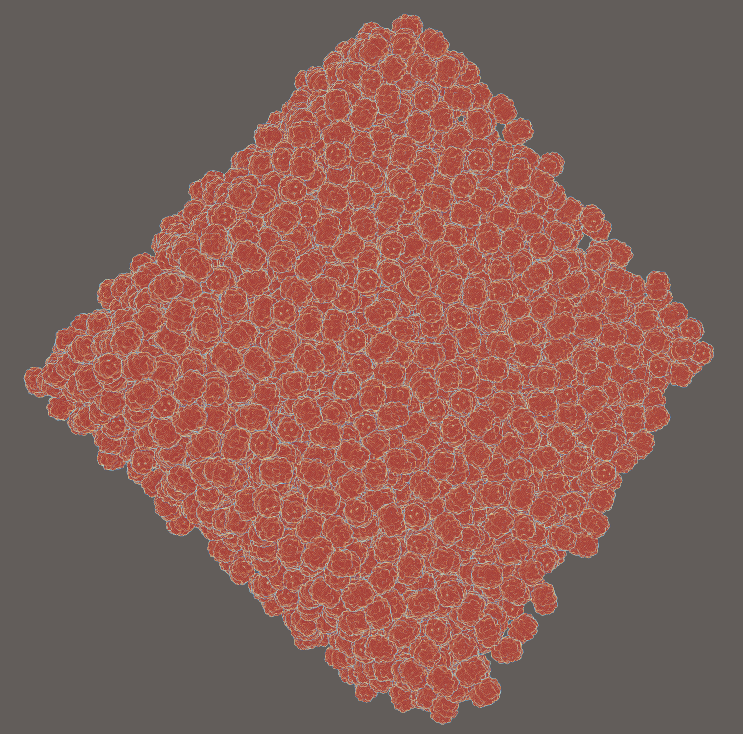
\includegraphics[width=0.5\textwidth]{archivos/tomo_occupany_breakdown.png}
        \caption{Tomograma sintético generado con la proteína \textit{2uv8\_10A.pns} en un volumen de $500\times500\times250$ vóxeles. Se alcanzó un grado de ocupancia del 32\% con 2\,552 monómeros insertados.}
        \label{fig:tomo-occupancy}
    \end{figure}
\end{enumerate}

\subsection{Fase 3: Implementación y Adaptación en PolNet}

Esta fase se centró en adaptar el algoritmo Tetris al \textit{framework} PolNet con el objetivo de facilitar una futura integración. En particular, fue necesario modificar el algoritmo para que tuviera en cuenta estructuras biológicas preexistentes, como membranas, durante el proceso de inserción de proteínas solubles y añadir una generación de clústeres inteligente.

\begin{enumerate}

     \item \textbf{Integración de elementos biológicos previo}: El algoritmo original asume un volumen inicialmente vacío; inicializa su \textit{output volume} a cero y empieza a insertar proteínas sin conocimiento de ninguna estructura preexistente. Para permitir la inserción de proteínas sobre membranas ya generadas por PolNet, se añadió una etapa de pre-carga que escribe las densidades de los elementos preexistentes directamente en el volumen de salida del algoritmo antes de comenzar la inserción:

    \begin{algorithm}[H]
        \caption{Pre-carga de membrana en el volumen Tetris}
        \label{alg:preload}
        \KwIn{Volumen MRC de membrana ($V_{mem}$), umbral proteico $\theta$}
        \KwOut{\textit{output\_volume} inicializado con regiones prohibidas}
        $allowed\_mask \gets \lnot(V_{mem} > 0)$ \tcp*{True = vóxel libre}
        $tetris.output\_volume \gets \mathbf{0}$ \tcp*{inicialización original}
        $tetris.output\_volume[\lnot allowed\_mask] \gets \infty$ \tcp*{nueva etapa: $\rho_{mem} \gg \theta$}
    \end{algorithm}

    Al asignar $\rho_{membrane} = 500.0 \gg \theta_{protein}$ a todos los vóxeles de membrana, estos son detectados como «ocupados» por el mecanismo de colisión del algoritmo en todas las iteraciones posteriores, sin necesidad de modificar la lógica interna de inserción. Adicionalmente, la \textit{allowed\_mask} binaria se propaga a la función de correlación para penalizar con $-10^9$ cualquier candidato de inserción que caiga sobre un vóxel de membrana. Esto garantiza que la inserción de proteínas solubles se limite a regiones biológicamente permitidas, independientemente de la intensidad local de la correlación.

    \item \textbf{Sistema de semillas inteligente y generación de clústeres}: El algoritmo original coloca la primera molécula en el centro del volumen y luego crece por proximidad, dejando los bordes del tomograma vacíos y sin tener en cuenta otros elementos. Se desarrolló una función \texttt{pick\_seed()} que muestrea uniformemente posiciones válidas en todo el espacio libre viable:
    \begin{equation}
    \text{viable}[z, y, x] = \text{allowed}[z, y, x] \land (\text{output}[z, y, x] \leq \theta) \land (z, y, x \notin \text{border})
    \end{equation}

    donde $\text{border}$ denota la región de margen ($\lfloor box\_size/2 \rfloor$ vóxeles desde cada borde), garantizando que la proteína quepa íntegra. Su funcionamiento se detalla en el Algoritmo~\ref{alg:pick_seed}:

    \begin{algorithm}[H]
        \caption{\texttt{pick\_seed}: muestreo uniforme de semilla válida}
        \label{alg:pick_seed}
        \KwIn{$allowed\_mask$, $output\_volume$, umbral $\theta$, $box\_size$}
        \KwOut{Coordenada semilla $(z,y,x)$ o $\varnothing$}
        $half \gets \lfloor box\_size / 2 \rfloor$\;
        $empty \gets allowed\_mask \land (output\_volume \leq \theta)$\;
        $viable \gets \{(z,y,x) \in empty : half \leq z < D_z{-}half,\; half \leq y < D_y{-}half,\; half \leq x < D_x{-}half\}$\;
        \If{$viable = \varnothing$}{\Return $\varnothing$}
        \Return coordenada aleatoria uniforme de $viable$\;
    \end{algorithm}

    El mecanismo de crecimiento de clústeres combina \texttt{pick\_seed()} con un contador de fallos consecutivos controlado por el parámetro  \texttt{$T_{cluster}$} (fijado a 10). El Algoritmo~\ref{alg:cluster} describe el bucle de inserción para cada tipo de proteína:

    \begin{algorithm}[H]
        \caption{Crecimiento de clúster guiado por semilla}
        \label{alg:cluster}
        \KwIn{$allowed\_mask$, $output\_volume$, proteína $M$, $\theta$, $T_{cluster} = 10$}
        \KwOut{Proteínas insertadas en el volumen}
        $target \gets \texttt{pick\_seed}(allowed\_mask, output, \theta, box\_size)$\;
        $failures \gets 0$\;
        \While{$failures < T_{cluster}$}{
            \If{$target = \varnothing$}{\textbf{break}\;}
            $rotated \gets \texttt{randomly\_rotate}(M)$\;
            $M_{bin} \gets \texttt{smooth\_and\_binarize}(rotated,\; \sigma{=}1.5,\; \theta)$\;
            $template \gets \texttt{create\_in\_shell}(M_{bin},\; r{=}(0,2),\; penalty{=}100)$\;
            $result \gets \texttt{insert\_molecule\_3d}(template, rotated, target)$\;
            \eIf{$result = \texttt{inserted}$}{
                $failures \gets 0$\;
                $target \gets$ última posición insertada \tcp*{crecimiento local}
            }{
                $failures \gets failures + 1$\;
                $target \gets \texttt{pick\_seed}(\dots)$ \tcp*{nueva semilla global}
            }
        }
    \end{algorithm}

    Este diseño produce un empaquetamiento en dos niveles: cuando la inserción es exitosa, el algoritmo continúa en la misma región (\textit{crecimiento local}), favoreciendo clústeres compactos; cuando falla, se muestrea una nueva semilla aleatoria del espacio global (\textit{reset global}), evitando que el algoritmo quede atrapado en zonas saturadas. El proceso finaliza al acumular $T_{cluster}$ fallos consecutivos para el tipo de proteína en curso, momento en el que el algoritmo pasa al siguiente tipo.

    \item \textbf{Gestión de umbrales y selección de proteínas}: Para garantizar la consistencia en la detección de colisiones, se establece un umbral de binarización global definido como el 8\%  del menor valor máximo de densidad entre todas las proteínas del catálogo de entrada:
    \begin{equation}
        \theta = 0.08 \cdot \min_{i \in \text{catálogo}} \left( \max(\rho_i) \right)
    \end{equation}
   
    El umbral del 8\% fue determinado empíricamente (aunque en \texttt{SAWCL} se establece al 10\%) como el valor mínimo que garantiza que todos los tipos proteicos presenten al menos algunos vóxeles por encima del umbral tras la binarización, evitando que las moléculas de menor intensidad queden silenciadas. Este umbral se mantiene constante y único para todas las iteraciones del algoritmo: si cada tipo de proteína usara su propio umbral, una macromolécula con umbral bajo podría solaparse geométricamente con zonas ya marcadas como ocupadas por otra de umbral mayor, produciendo fallos en la detección de colisiones.
    
    El algoritmo de selección prioriza la inserción de las proteínas de mayor tamaño para maximizar el empaquetamiento inicial y reducir la fragmentación temprana del volumen libre. El tamaño se determina mediante la \textit{ocupación interna} de cada proteína, definida como:

    \begin{equation}
        \text{Ocupación}_{\text{interna}} = \frac{\text{Vóxeles}_{\text{ocupados}}}{\text{Volumen}_{\text{total}}}
    \end{equation}

    Donde los \textit{vóxeles ocupados} son los que superan el umbral de binarización. Por ejemplo, para la proteína \textit{5mrc\_10A} con dimensiones de caja de ($72 \times 72 \times 72$), el volumen total es de $373{,}248$ vóxeles. Al ocupar $7{,}599$  vóxeles efectivos, su ocupación interna es del $2.04\%$.

    \item \textbf{Consistencia de proteínas solubles}: Se añadió una comprobación explícita de integridad geométrica (\textit{boundary check}) que verifica si la caja delimitadora de la molécula candidata excede los límites del volumen:
    \begin{equation}
    \text{válido} \Leftrightarrow (z - r/2 \geq 0) \land (z + r/2 < D_z) \land (y - r/2 \geq 0) \land (y + r/2 < D_y) \land \dots
    \end{equation}

    Si la comprobación falla (el \textit{c-map} indica buen contacto pero no garantiza ausencia de solapamiento vóxel a vóxel), la posición correspondiente en el \textit{c-map} se penaliza con $-10^9$, descartándola como candidato. El algoritmo continúa evaluando las siguientes posiciones de mayor correlación dentro del mismo mapa, con un máximo de 50 intentos por llamada. Si ninguna posición supera todas las comprobaciones, el algoritmo devuelve \texttt{'saturated'}, indicando que no existe espacio viable en la región local analizada.

        \item \textbf{Análisis de rendimiento de la implementación adaptada}: Con todas las modificaciones integradas —pre-carga de membrana, \texttt{pick\_seed} con muestreo uniforme y bucle de crecimiento de clústeres— se procedió a medir empíricamente el tiempo real de cada etapa. El tiempo de validación e inserción se obtiene como:
    \begin{equation}
        t_{\textit{insert\_validation}} = t_{\textit{insert\_molecule\_3d}} - t_{\textit{fft\_correlation}}
    \end{equation}

   El experimento se realizó sobre un volumen de $500\times500\times250$ vóxeles con una
    membrana preexistente cuya ocupancia es del \textbf{11.54\%}. Se empleó la proteína
    \textit{2uv8\_10A.pns}, alcanzando una ocupancia final del \textbf{26.56\%} con
    \textbf{1\,184 monómeros insertados} en un tiempo total de \textbf{191.84\,s}.
    La Figura~\ref{fig:profile-breakdown} muestra la curva de ocupancia frente al tiempo,
    con el área bajo la curva coloreada según la etapa dominante en cada tramo.
    
    \begin{figure}[H]
        \centering
        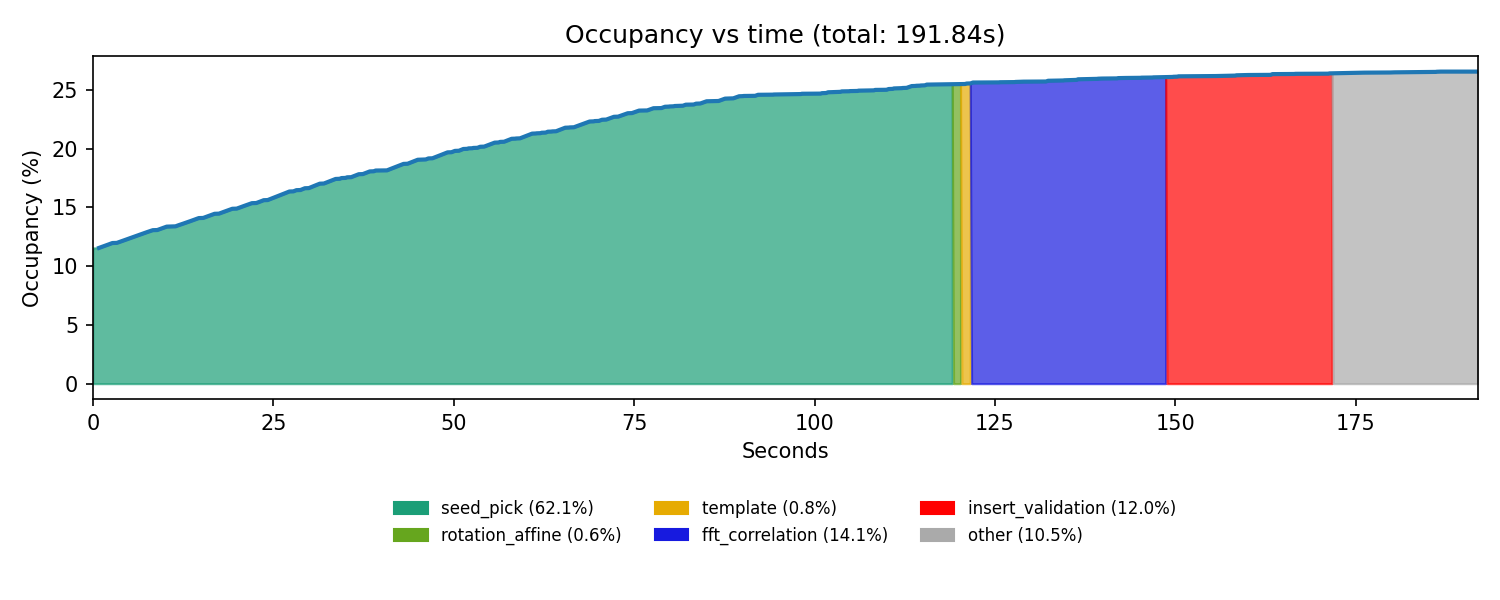
\includegraphics[width=1\textwidth]{archivos/profile_occupancy_breakdown-cpu.png}
        \caption{Tiempo de ejecución en CPU por etapa del algoritmo Tetris. El área coloreada
        bajo la curva de ocupancia indica el tiempo acumulado de cada operación.}
        \label{fig:profile-breakdown}
    \end{figure}
    
    Los resultados, resumidos en la Tabla~\ref{tab:profile}, revelan que \texttt{pick\_seed}
    es el componente de mayor carga computacional, representando el \textbf{62.1\%} del tiempo
    total (119.10\,s). A continuación se sitúan la correlación FFT~3D con un \textbf{14.1\%}
    (27.06\,s) y la validación e inserción con un \textbf{12.0\%} (23.02\,s). El
    \textbf{10.5\%} restante corresponde a operaciones misceláneas de Python e I/O. Las
    operaciones de generación de \textit{in-shell} y rotación afín resultan prácticamente
    despreciables ($<2\%$ combinadas).
    
    \begin{table}[H]
    \centering
    \begin{tabular}{|l|r|r|}
    \hline
    \textbf{Operación} & \textbf{Tiempo (s)} & \textbf{Porcentaje} \\
    \hline
    Selección de semilla (\texttt{pick\_seed}) & 119.10 & 62.1\% \\
    Correlación FFT 3D                         &  27.06 & 14.1\% \\
    Validación e inserción                     &  23.02 & 12.0\% \\
    Otros (Python, I/O)                        &  20.06 & 10.5\% \\
    Generación \textit{in-shell}               &   1.48 &  0.8\% \\
    Rotación afín                              &   1.12 &  0.6\% \\
    \hline
    \textbf{Total}                             & \textbf{191.84} & \textbf{100\%} \\
    \hline
    \end{tabular}
    \caption{Desglose del tiempo de ejecución en CPU de cada operación durante la inserción Tetris.}
    \label{tab:profile}
    \end{table}
    
    Estos datos orientan la estrategia de optimización en dos direcciones: (1)~la aceleración
    GPU reduce el coste de la correlación FFT y la validación mediante paralelismo masivo;
    (2)~la función \texttt{pick\_seed} se beneficia igualmente del backend \texttt{CuPy},
    que ejecuta el \texttt{argwhere} sobre el volumen completo en paralelo, eliminando el
    principal cuello de botella identificado.

    \item \textbf{Esquema final:} Finalmente el algoritmo Tetris queda modificado de la siguiente forma:

    \begin{figure}[H]
        \centering
        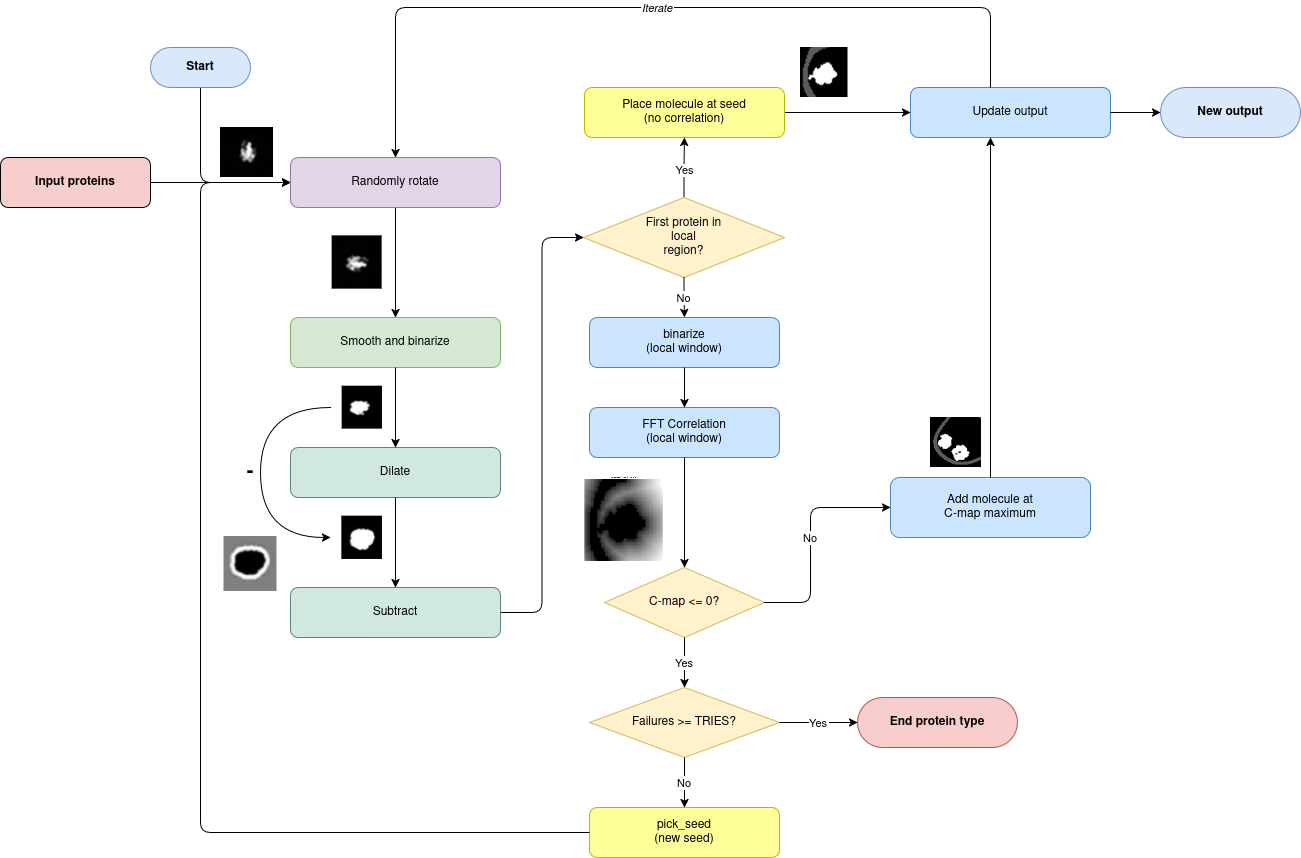
\includegraphics[width=0.7\textwidth]{archivos/tetris-new.png}
        \caption{Diagrama de flujo del algoritmo Tetris modificado.}
        \label{fig:tetris-new}
    \end{figure}
    
    El diagrama ilustra el flujo completo del algoritmo de inserción de proteínas Tetris. A partir de las proteínas de entrada, cada iteración comienza con una rotación aleatoria del volumen molecular, seguida de un suavizado y binarización para obtener una representación binaria de la molécula. A continuación, se generan dos dilataciones del volumen binarizado (exterior e interior) y se restan para construir el \textit{in-shell template}, que codifica la superficie de la proteína con valores positivos en el shell y penalización negativa en el núcleo.
    
    La inserción se delega a \texttt{insert\_molecule\_3d}, que extrae una ventana local alrededor del \textit{seed} seleccionado por \texttt{pick\_seed}. Si la región local está completamente vacía (primera proteína en esa zona) y hay espacio para ella, la molécula se coloca directamente en el \textit{seed} sin necesidad de correlación. En caso contrario, se binariza la ventana local y se realiza una correlación FFT entre dicha ventana y el \textit{in-shell template}, obteniendo un mapa de correlación (C-map) que indica la traslación óptima para empaquetar la nueva proteína junto a las existentes. Si el máximo del C-map es negativo (ninguna posición válida disponible), se incrementa el contador de fallos; al alcanzar el límite \texttt{$T_{cluster}$}, se da por finalizada la inserción del tipo proteico actual. De lo contrario, se selecciona un nuevo \textit{seed} y se reitera el proceso. Tras una inserción exitosa, el volumen de salida se actualiza y el algoritmo itera desde la nueva posición.
    
    
\end{enumerate}

\subsection{Fase 4: Optimización mediante aceleración GPU}

Una vez verificada la corrección lógica de la implementación adaptada, se procedió a su optimización mediante computación paralela en GPU.

\begin{enumerate}
      \item \textbf{Identificación de operaciones paralelizables}: Las dos operaciones más costosas del algoritmo (como se observó antes) son \texttt{insert\_molecule\_3d} —método integrado que engloba la correlación FFT 3D y la validación de inserción, representando conjuntamente el 26.1\% del tiempo total— y \texttt{pick\_seed}, con un 62.1\%, cuyo \texttt{argwhere} sobre el volumen completo se beneficia directamente del paralelismo masivo de la GPU. Ambas operaciones cuentan con implementaciones optimizadas en \texttt{CuPy}. Las operaciones de rotación afín y filtrado gaussiano son computacionalmente despreciables ($<2\%$) pero también se redirigen al backend GPU para mantener los datos en memoria de dispositivo y evitar transferencias innecesarias.

    \item \textbf{Implementación de rutas duales CPU/GPU}: Se implementó un sistema de selección de backend controlado por el flag \texttt{USE\_GPU}. Si \texttt{USE\_GPU = True}, las operaciones se redirigen a las funciones equivalentes de \texttt{cupyx.scipy}; en caso contrario, el código funciona de forma transparente con \texttt{scipy} en CPU, sin cambios en la lógica algorítmica. La Figura~\ref{fig:esquema-gpu-cpu} ilustra este esquema de enrutamiento.


    \begin{figure}[H]
        \centering
        \includegraphics[width=0.65\textwidth]{archivos/esquema_gpu_cpu.png}
        \caption{Esquema de enrutamiento CPU/GPU.}
        \label{fig:esquema-gpu-cpu}
    \end{figure}

    En función de la disponibilidad de una GPU compatible con CUDA, las operaciones de correlación FFT, filtrado gaussiano, rotación afín y muestreo de semilla se ejecutan sobre \texttt{CuPy} (GPU) o \texttt{SciPy/NumPy} (CPU), manteniendo la misma lógica algorítmica en ambos casos.


    \item \textbf{Minimización de transferencias de memoria}: Las transferencias entre memoria principal (CPU) y memoria de la GPU son un cuello de botella conocido en computación heterogénea. Se optimizó el flujo para que cada operación GPU reciba datos NumPy, los convierta a \texttt{cupy.ndarray}, ejecute el cálculo en GPU, y devuelva el resultado de nuevo a NumPy, evitando transferencias intermedias innecesarias.

    \item \textbf{Análisis de rendimiento de la implementación GPU}: Bajo las mismas condiciones experimentales del perfilado CPU (volumen $500\times500\times250$, proteína \textit{2uv8\_10A.pns}, $26.5\%$ de ocupancia), se midió el tiempo de ejecución de la implementación GPU con el mismo script \texttt{profile\_test.py} instrumentado. Los resultados se recogen en la Tabla~\ref{tab:profile-gpu}.

    \begin{table}[H]
    \centering
    \begin{tabular}{|l|r|r|r|r|}
    \hline
    \textbf{Operación} & \textbf{CPU (s)} & \textbf{CPU (\%)} & \textbf{GPU (s)} & \textbf{GPU (\%)} \\
    \hline
    Selección de semilla (\texttt{pick\_seed}) & 119.10 & 62.1\% & 0.54  &  0.7\% \\
    Correlación FFT 3D                         &  27.06 & 14.1\% & 0.62  &  0.8\% \\
    Validación e inserción                     &  23.02 & 12.0\% & 41.36 & 52.3\% \\
    Otros (Python, I/O)                        &  20.06 & 10.5\% & 35.06 & 44.4\% \\
    Generación \textit{in-shell}               &   1.48 &  0.8\% &  1.12 &  1.4\% \\
    Rotación afín                              &   1.12 &  0.6\% &  0.34 &  0.4\% \\
    \hline
    \textbf{Total}                             & \textbf{191.84} & \textbf{100\%} & \textbf{79.04} & \textbf{100\%} \\
    \hline
    \end{tabular}
    \caption{Comparación del desglose de tiempo de ejecución entre las implementaciones CPU y GPU (volumen $500\times500\times250$, proteína \textit{2uv8\_10A.pns}, $26.56\%$ de ocupancia final). La GPU fue una NVIDIA RTX 4090.}
    \label{tab:profile-gpu}
    \end{table}

    La Figura~\ref{fig:profile-breakdown-gpu} muestra la curva de ocupancia frente al tiempo para la ejecución GPU, coloreada por etapa dominante, análoga a la Figura~\ref{fig:profile-breakdown} del perfil CPU.

    \begin{figure}[H]
        \centering
        \includegraphics[width=1\textwidth]{archivos/profile_occupancy_breakdown-gpu.png}
        \caption{Desglose del tiempo de ejecución por etapa de la implementación GPU del algoritmo Tetris. El área coloreada bajo la curva de ocupancia indica el tiempo acumulado de cada operación (experimento: volumen $500\times500\times250$, proteína \textit{2uv8\_10A.pns}, 26.56\% de ocupancia final , NVIDIA RTX 4090).}
        \label{fig:profile-breakdown-gpu}
    \end{figure}

     Los resultados confirman una aceleración global de $\times$\textbf{2.43} (191.84\,s $\to$ 79.04\,s). El beneficio más notable es la eliminación práctica de los dos cuellos de botella originales: \texttt{pick\_seed} pasa de 119.10\,s (62.1\%) a 0.54\,s (0.7\%) gracias al \texttt{argwhere} paralelo de \texttt{CuPy}, y la correlación FFT 3D se reduce de 27.06\,s (14.1\%) a 0.62\,s (0.8\%) mediante \texttt{cupyx.scipy.signal.correlate}. El tiempo restante —validación e inserción (41.36\,s) y otros (35.06\,s)— constituye el piso de tiempo de ejecución inherente al algoritmo: son operaciones de control secuencial, comprobaciones de colisión y gestión del estado interno que no son paralelizables y cuyo coste es equivalente al de la I/O en sistemas convencionales. Este suelo no es reducible mediante aceleración hardware adicional sin un rediseño algorítmico profundo, por lo que la implementación GPU puede considerarse próxima al límite de rendimiento alcanzable con la arquitectura actual.
    
    
\end{enumerate}

\subsection{Fase 5: Evaluación experimental comparativa}

Esta fase cierra la metodología y da paso al Capítulo de Resultados. El objetivo es comparar cuantitativamente Tetris frente a SAWLC bajo las mismas condiciones experimentales. Todos los experimentos utilizan el mismo conjunto de \textbf{11 proteínas solubles} a resolución de 10\,\AA\ (detalladas en el Anexo) y un volumen de membrana real de dimensiones $500\times500\times250$ vóxeles. Las herramientas se organizan en la carpeta \texttt{benchmark/}:

\begin{enumerate}
    \item \textbf{\texttt{profile\_test.py}} — Perfilado por fases de Tetris (CPU o GPU según \texttt{USE\_GPU}). Instrumenta el algoritmo con temporizadores finos y genera una gráfica de ocupancia vs tiempo coloreada por etapa (selección de semilla, rotación, \textit{in-shell}, correlación FFT, validación). Permite identificar qué operaciones dominan el tiempo de ejecución.

    \item \textbf{\texttt{profile\_comparison.py}} — Curva de ocupancia acumulada de los tres algoritmos (Tetris CPU, Tetris GPU y SAWLC) ejecutados secuencialmente sobre el mismo volumen con las 11 proteínas. Produce una gráfica de líneas y un CSV. El objetivo es comparar la velocidad a la que cada algoritmo llena el volumen disponible.

    \item \textbf{\texttt{benchmark\_scientific\_comparison.py}} — Barrido sistemático de targets de ocupancia del 2.5\% al 70\% en pasos de 2.5\%, ejecutando ambos algoritmos en cada punto con caché JSON. Genera 4 gráficas: ocupancia alcanzada vs objetivo, tiempo de ejecución, throughput, y fallos de SAWLC. Permite caracterizar el rendimiento en todo el espectro de densidad.

    \item \textbf{\texttt{sawlc-cpu-gpu/plot\_comparison.py}} — Genera una figura de 4 paneles a partir de logs reales (una ejecución por número de tipos de proteína activos, de 1 a 11): ocupancia total, tiempo de ejecución, población de monómeros por tipo (barras apiladas) y throughput en función de la diversidad molecular.
\end{enumerate}

Las métricas registradas en todos los experimentos son: tiempo de ejecución ($t$), ocupancia de proteínas ($\rho_{prot}$), ocupancia total ($\rho_{total}$), número de monómeros insertados, throughput (monómeros/minuto) y speedup ($t_{SAWLC}/t_{Tetris}$).\\

Esta metodología de cinco fases permitió: (1) establecer un entorno reproducible, (2) comprender el algoritmo de referencia, (3) adaptarlo al contexto de PolNet, (4) optimizarlo mediante GPU, y (5) validarlo experimentalmente frente a SAWLC.


